\documentclass[compress]{beamer}
\usepackage{ifthen,verbatim}

\newcommand{\isnote}{}
\xdefinecolor{lightyellow}{rgb}{1.,1.,0.25}
\xdefinecolor{darkblue}{rgb}{0.1,0.1,0.7}

%% Uncomment this to get annotations
%% \def\notes{\addtocounter{page}{-1}
%%            \renewcommand{\isnote}{*}
%% 	   \beamertemplateshadingbackground{lightyellow}{white}
%%            \begin{frame}
%%            \frametitle{Notes for the previous page (page \insertpagenumber)}
%%            \itemize}
%% \def\endnotes{\enditemize
%% 	      \end{frame}
%%               \beamertemplateshadingbackground{white}{white}
%%               \renewcommand{\isnote}{}}

%% Uncomment this to not get annotations
\def\notes{\comment}
\def\endnotes{\endcomment}

\setbeamertemplate{navigation symbols}{}
\setbeamertemplate{headline}{\mbox{ } \hfill
\begin{minipage}{5.5 cm}
\vspace{-0.75 cm} \small
\end{minipage} \hfill
\begin{minipage}{4.5 cm}
\vspace{-0.75 cm} \small
\begin{flushright}
\ifthenelse{\equal{\insertpagenumber}{0}}{}{Jim Pivarski \hspace{0.2 cm} \insertpagenumber\isnote/\pageref{numpages}}
\end{flushright}
\end{minipage}\mbox{\hspace{0.2 cm}}\includegraphics[height=1 cm]{../cmslogo} \hspace{0.1 cm} \includegraphics[height=1 cm]{../tamulogo} \hspace{0.01 cm} \vspace{-1.05 cm}}

\begin{document}
%% \begin{frame}
%% \vfill
%% \begin{center}
%% \textcolor{darkblue}{\Large TITLE}

%% \vfill
%% \begin{columns}
%% \column{0.3\linewidth}
%% \begin{center}
%% \large
%% \textcolor{darkblue}{Jim Pivarski}

%% \vspace{0.2 cm}
%% Alexei Safonov
%% \end{center}

%% \column{0.3\linewidth}
%% \begin{center}
%% \large
%% K\'aroly Banicz
%% \end{center}
%% \end{columns}

%% \begin{columns}
%% \column{0.3\linewidth}
%% \begin{center}
%% \scriptsize
%% {\it Texas A\&M University}
%% \end{center}
%% \column{0.3\linewidth}
%% \begin{center}
%% \scriptsize
%% {\it US-CMS}
%% \end{center}
%% \end{columns}

%% \vfill
%% 31 March, 2009

%% \end{center}
%% \end{frame}

%% \begin{notes}
%% \item This is the annotated version of my talk.
%% \item If you want the version that I am presenting, download the one
%% labeled ``slides'' on Indico (or just ignore these yellow pages).
%% \item The annotated version is provided for extra detail and a written
%% record of comments that I intend to make orally.
%% \item Yellow notes refer to the content on the {\it previous} page.
%% \item All other slides are identical for the two versions.
%% \end{notes}

\small

\begin{frame}
\frametitle{New alignment of $\phi_y$ angles}

\begin{itemize}
\item This is the rotation angle of chambers in the transverse \mbox{plane of CMS\hspace{-1 cm}}
\item Important for $p_T$ and $q$ measurement (rotational analogue of local $x$ translations)
\item Alignment method inspired by $\vec{B}$-field measurements: track-minus-segment angle residuals
\item \textcolor{red}{Positive $q$ is red,} negative $q$ is black: we see 4~mrad \mbox{misalignment here\hspace{-1 cm}}
\end{itemize}

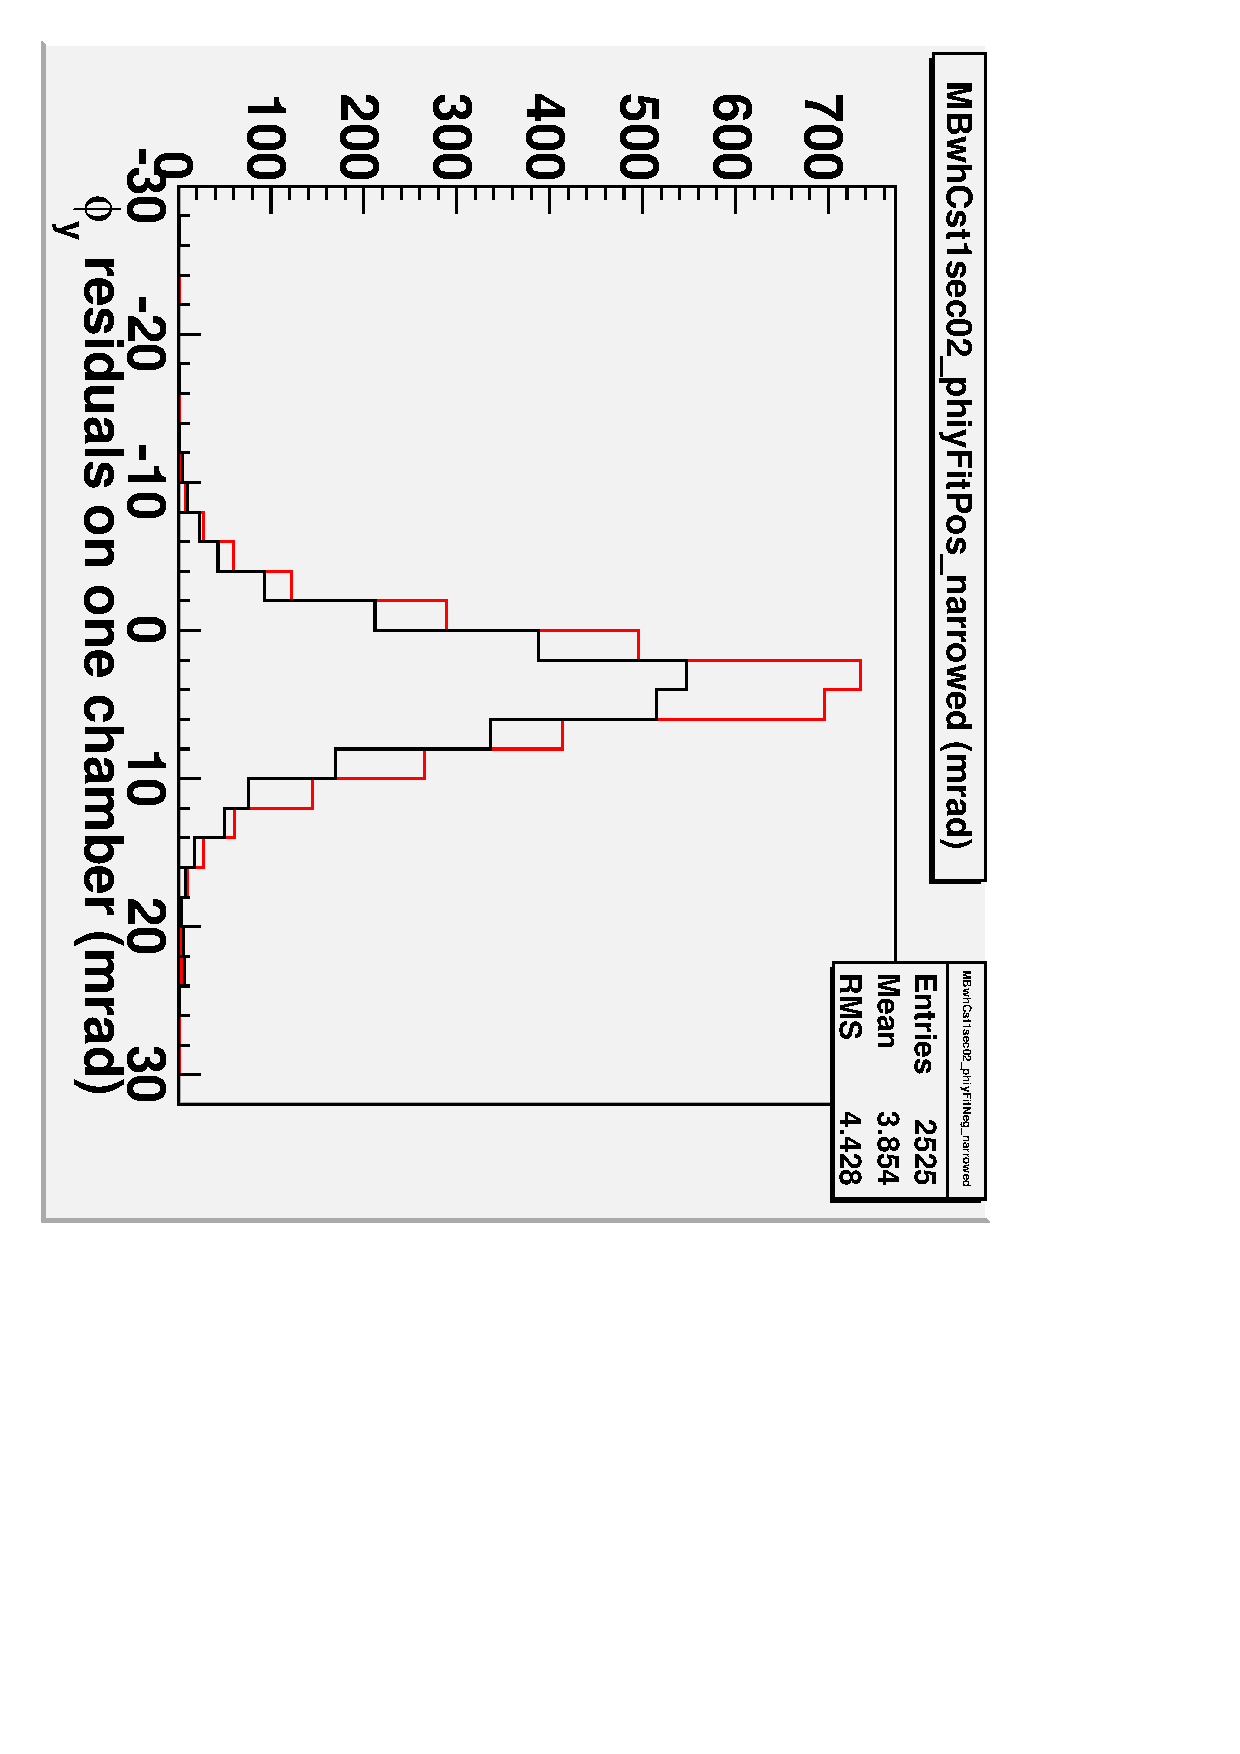
\includegraphics[height=0.5\linewidth, angle=90]{example_phiy.pdf} \mbox{\hspace{0.5 cm}} 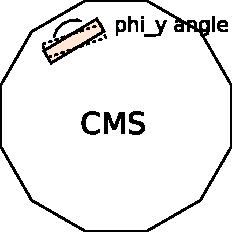
\includegraphics[width=0.37\linewidth]{what_phiy_is.pdf}
\end{frame}

\begin{frame}
\frametitle{New alignment fits}

\begin{itemize}
\item Combined fit to local $x$ (top left), sawtooth correlation (top
  right), local $z$ (bottom left), and $\phi_z$ (bottom right)
\item Data are projections (simple profiles), line is hyperplane of fit crest
\begin{itemize}
\item intersection with zero is not necessarily the mean (why we fit)
\item that's why top-right doesn't go through points
\end{itemize}
\end{itemize}

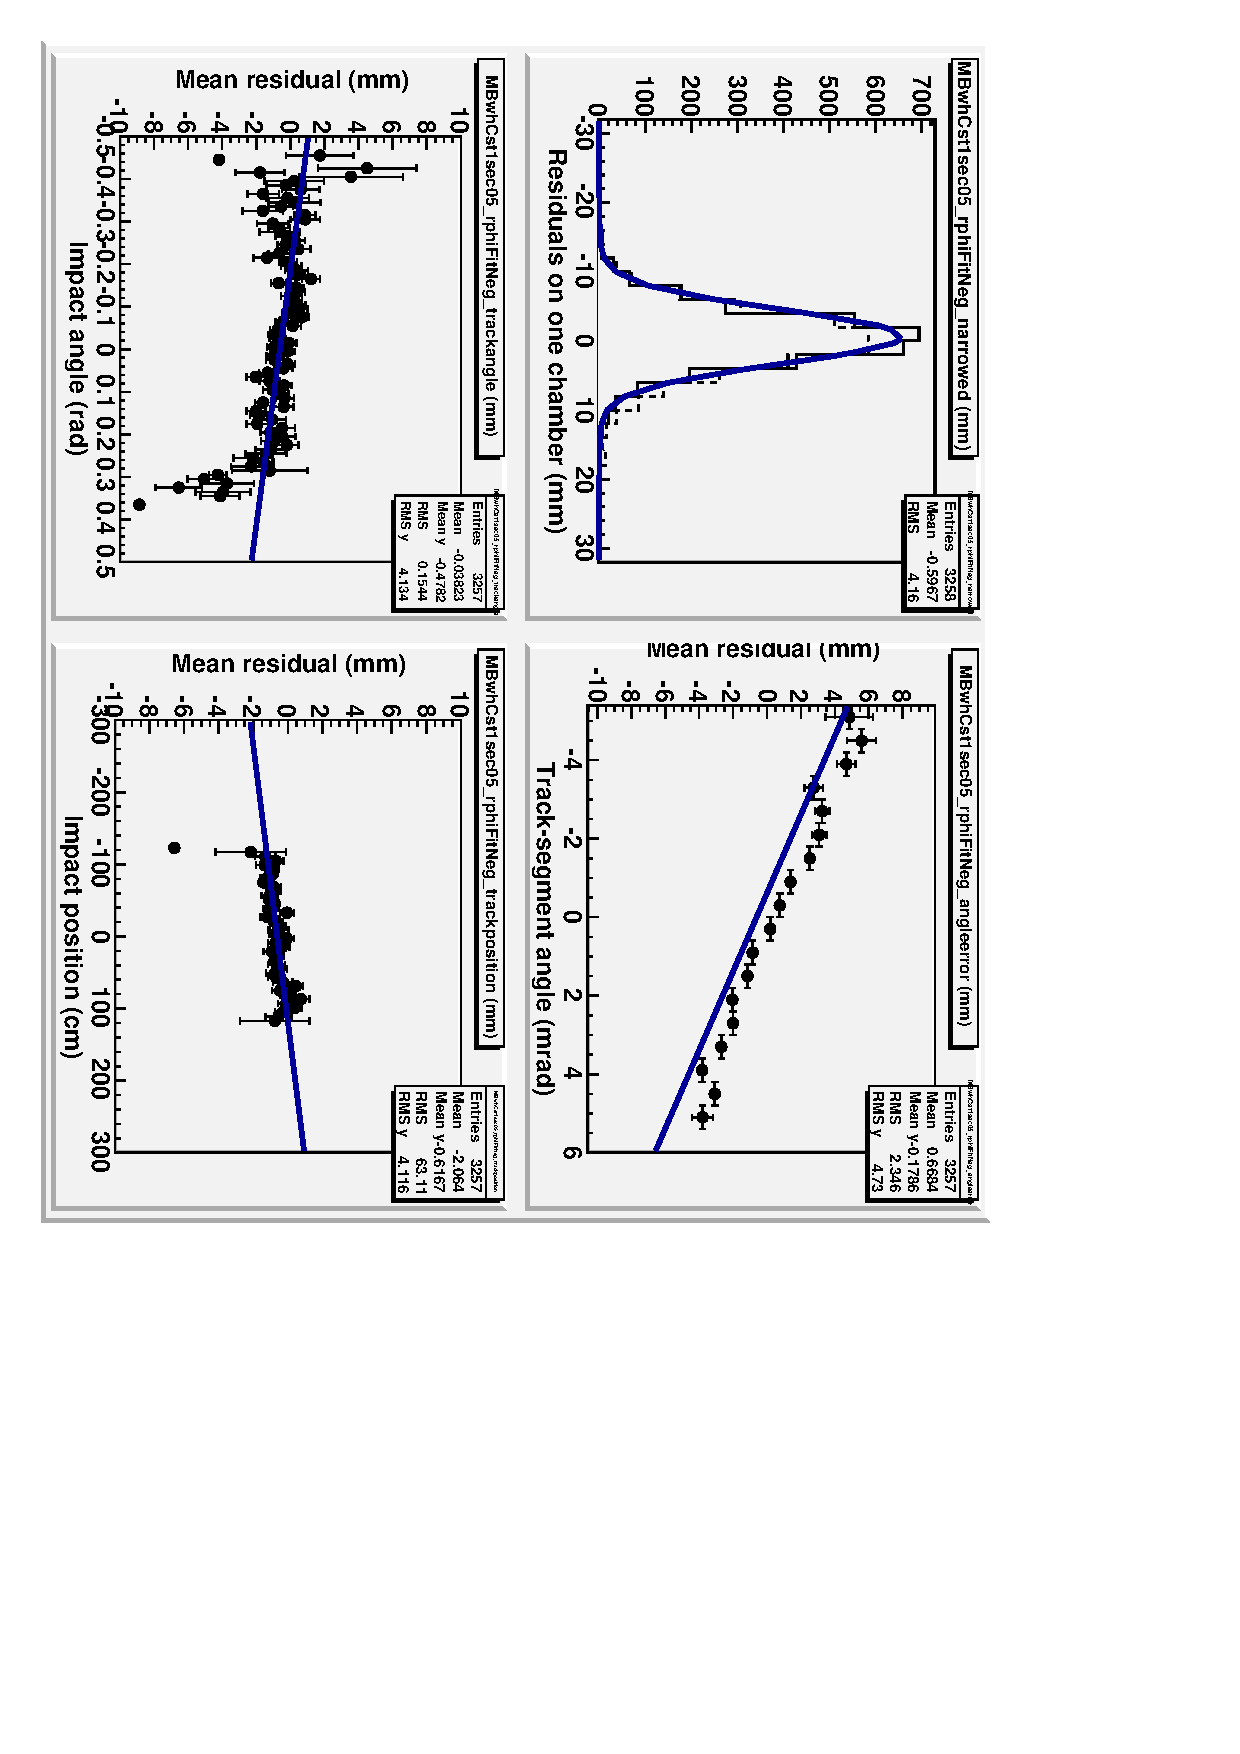
\includegraphics[height=0.7\linewidth, angle=90]{example_fit.pdf}
\end{frame}

\begin{frame}
\frametitle{CSC example, for fun}
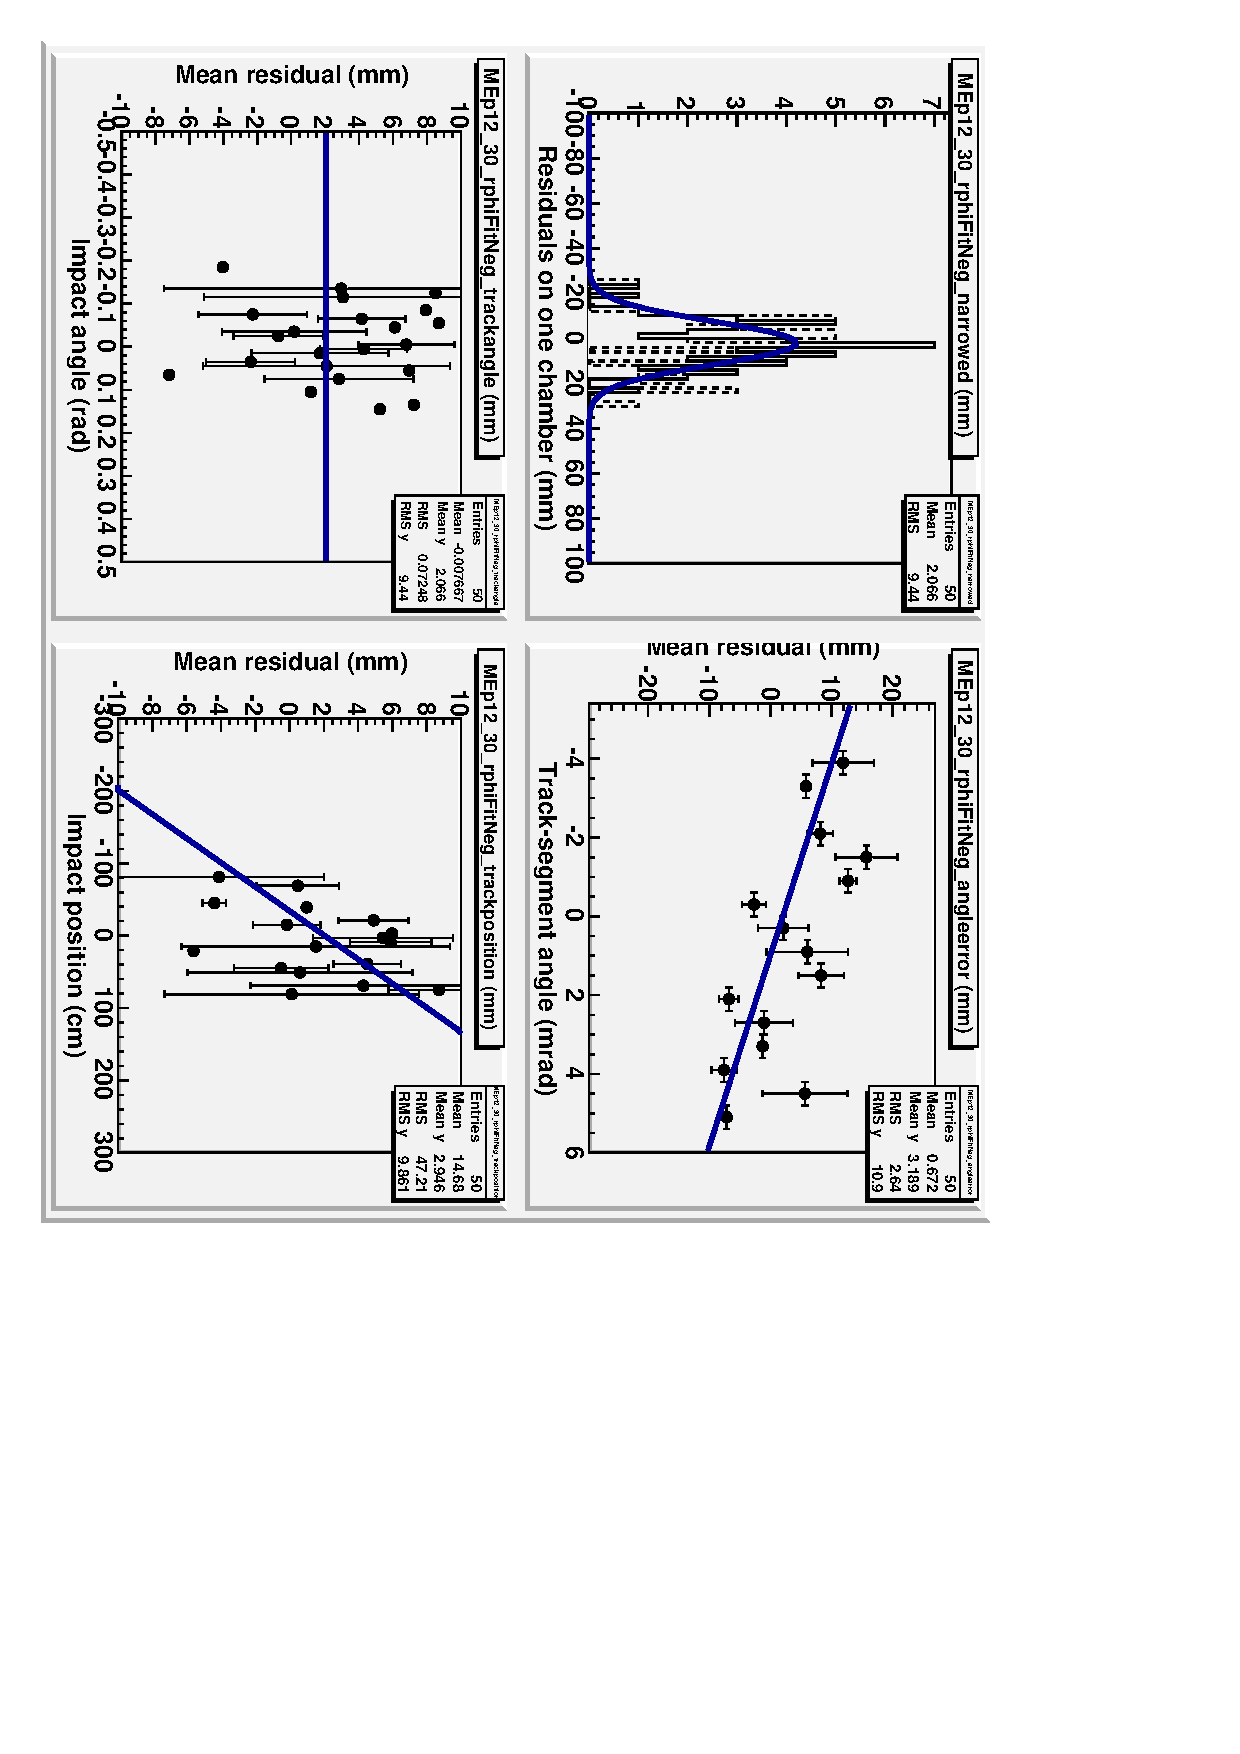
\includegraphics[height=0.7\linewidth, angle=90]{example_CSC.pdf}

\begin{itemize}
\item We can fix fit parameters (such as bottom-left, here)
\item Real CSC alignment will come from tracker $\to$ barrel $\to$ \mbox{endcap method\hspace{-1 cm}}
\item Good to know that the machinery will work \mbox{(more extensive MC tests)\hspace{-1 cm}}
\end{itemize}
\end{frame}

\begin{frame}
\frametitle{Interesting discovery}

\begin{itemize}
\item These are $\phi_y$ corrections as a function of $\phi$ around CMS \\ (dashed lines are the chamber boundaries)
\item Not due to acoplanarity: that would be $\phi_y$ vs.~local~$y$ (not seen)
\item Likely related to the famous ``sawtooth'' effect: sawtooth was shown to be related to track-minus-segment residuals ($\phi_y$ error)
\item Might be physically caused by superlayer~3 being wider than superlayer~1 (that's {\it only} a hypothesis!)
\end{itemize}

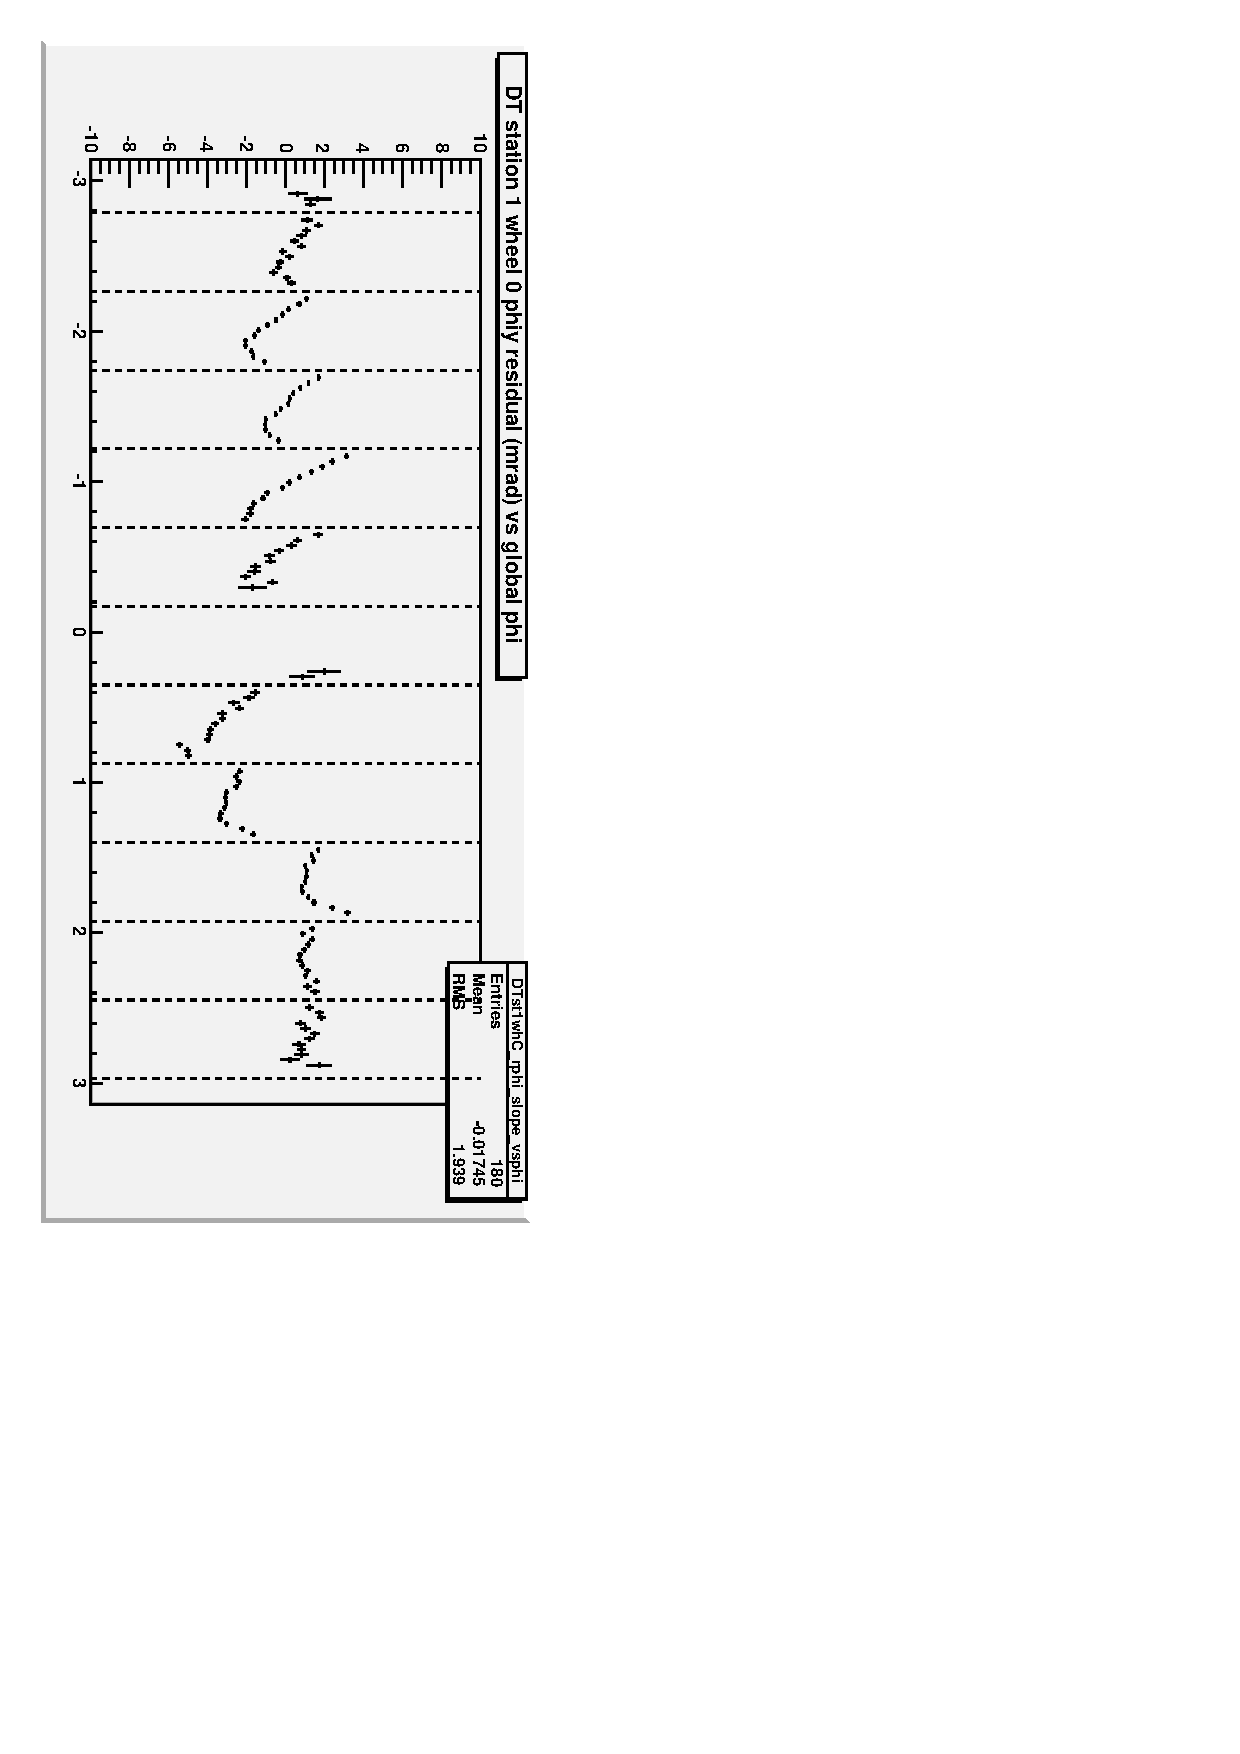
\includegraphics[height=\linewidth, angle=90]{possible_acoplanarity.pdf}
\end{frame}

\begin{frame}
\frametitle{Is it real?}

\begin{itemize}
\item Turn off the fancy fitting: do we see it with a simple profile
  plot? (each bin is just a mean, each error bar is just
  RMS/$\sqrt{N}$)
\item Yes, we see the same trends
\item RMS is huge because distribution has long non-Gaussian
  tails (that's why we do fancy fitting)
\end{itemize}

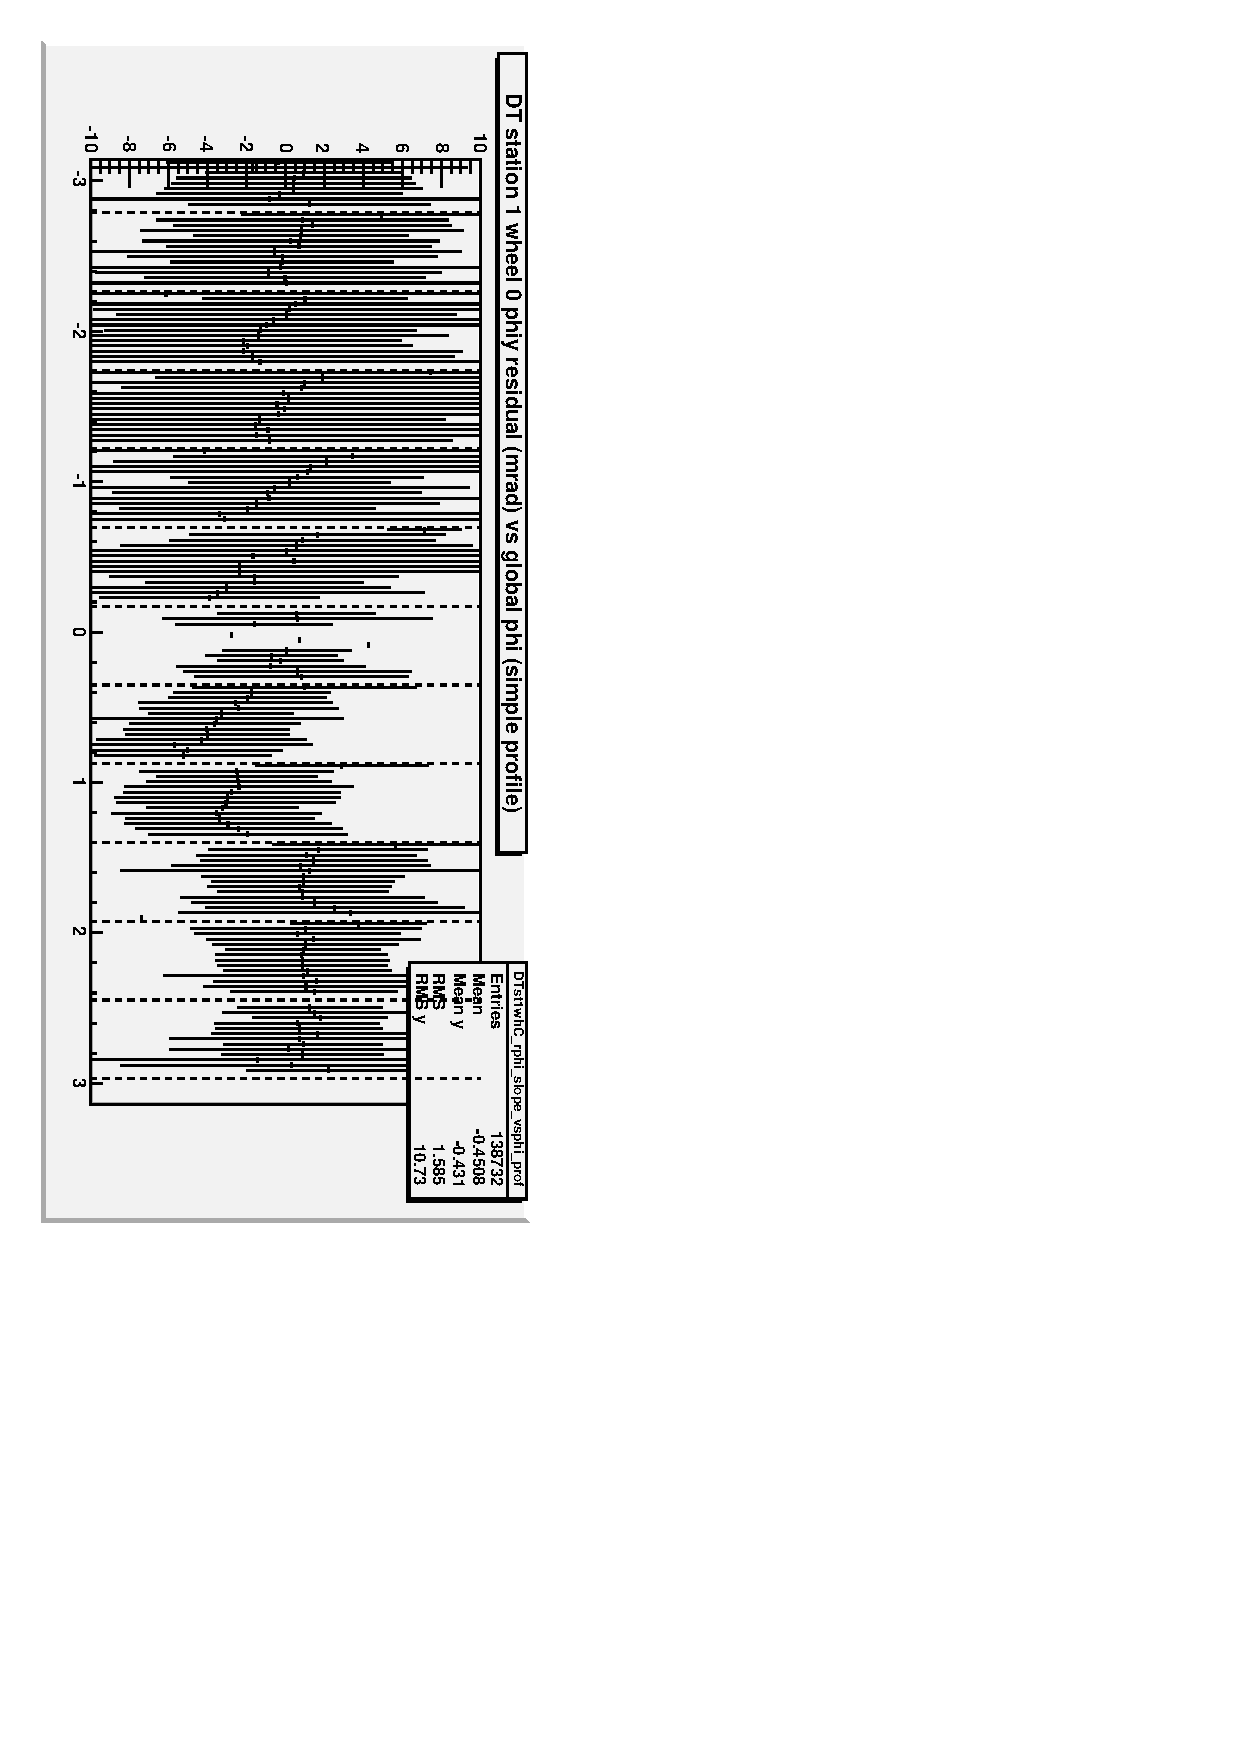
\includegraphics[height=\linewidth, angle=90]{possible_acoplanarity2.pdf}
\end{frame}

\begin{frame}
\frametitle{What about $\vec{B}$?}

\begin{itemize}
\item $\phi_y$ angles are used to measure $\vec{B}$: is that an issue here?
\item This is the $(R_+ - R_-)/2$ antisymmetric part: no trend at all
\end{itemize}

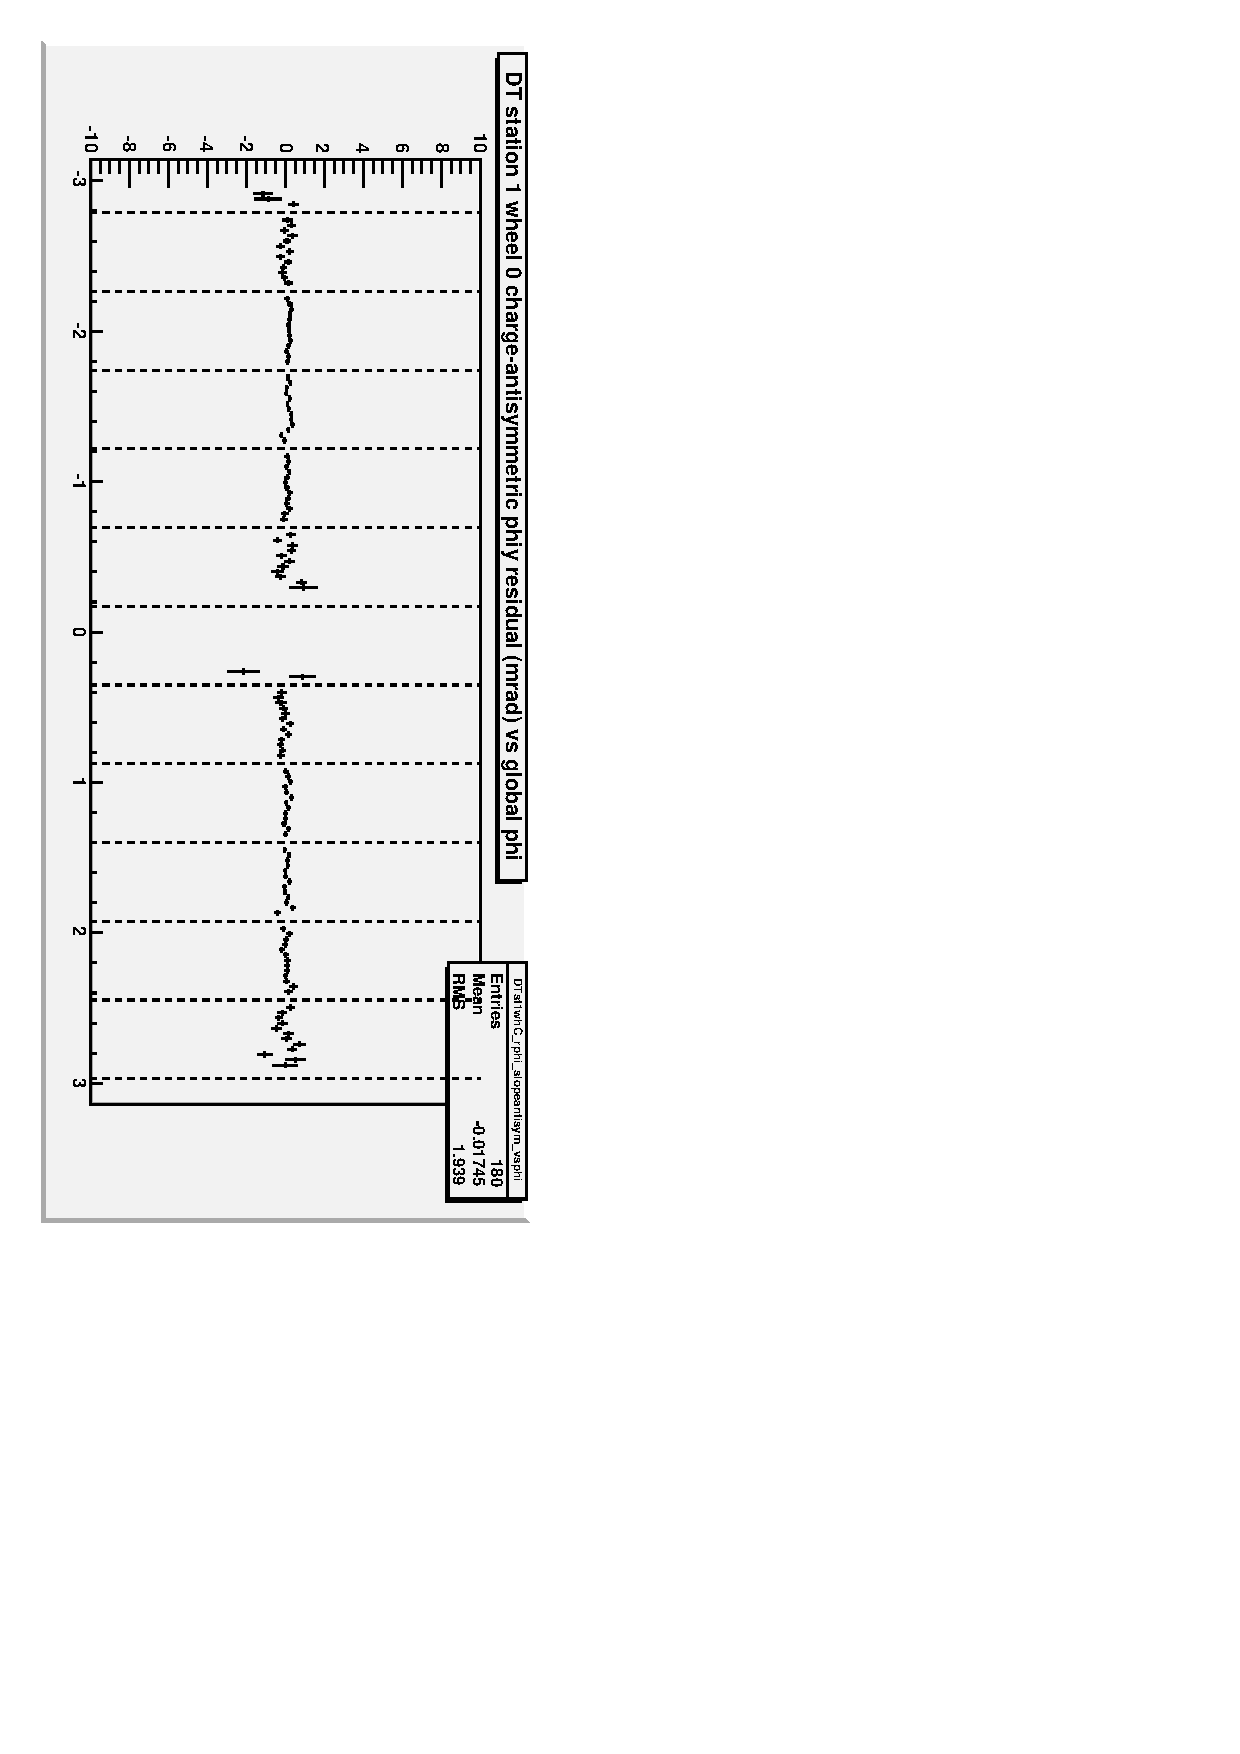
\includegraphics[height=\linewidth, angle=90]{possible_acoplanarity3.pdf}
\end{frame}

\begin{frame}
\frametitle{Do we see it in MC?}

\begin{itemize}
\item Collisions MC, used to tune and debug the software
\item No trend at all
\end{itemize}

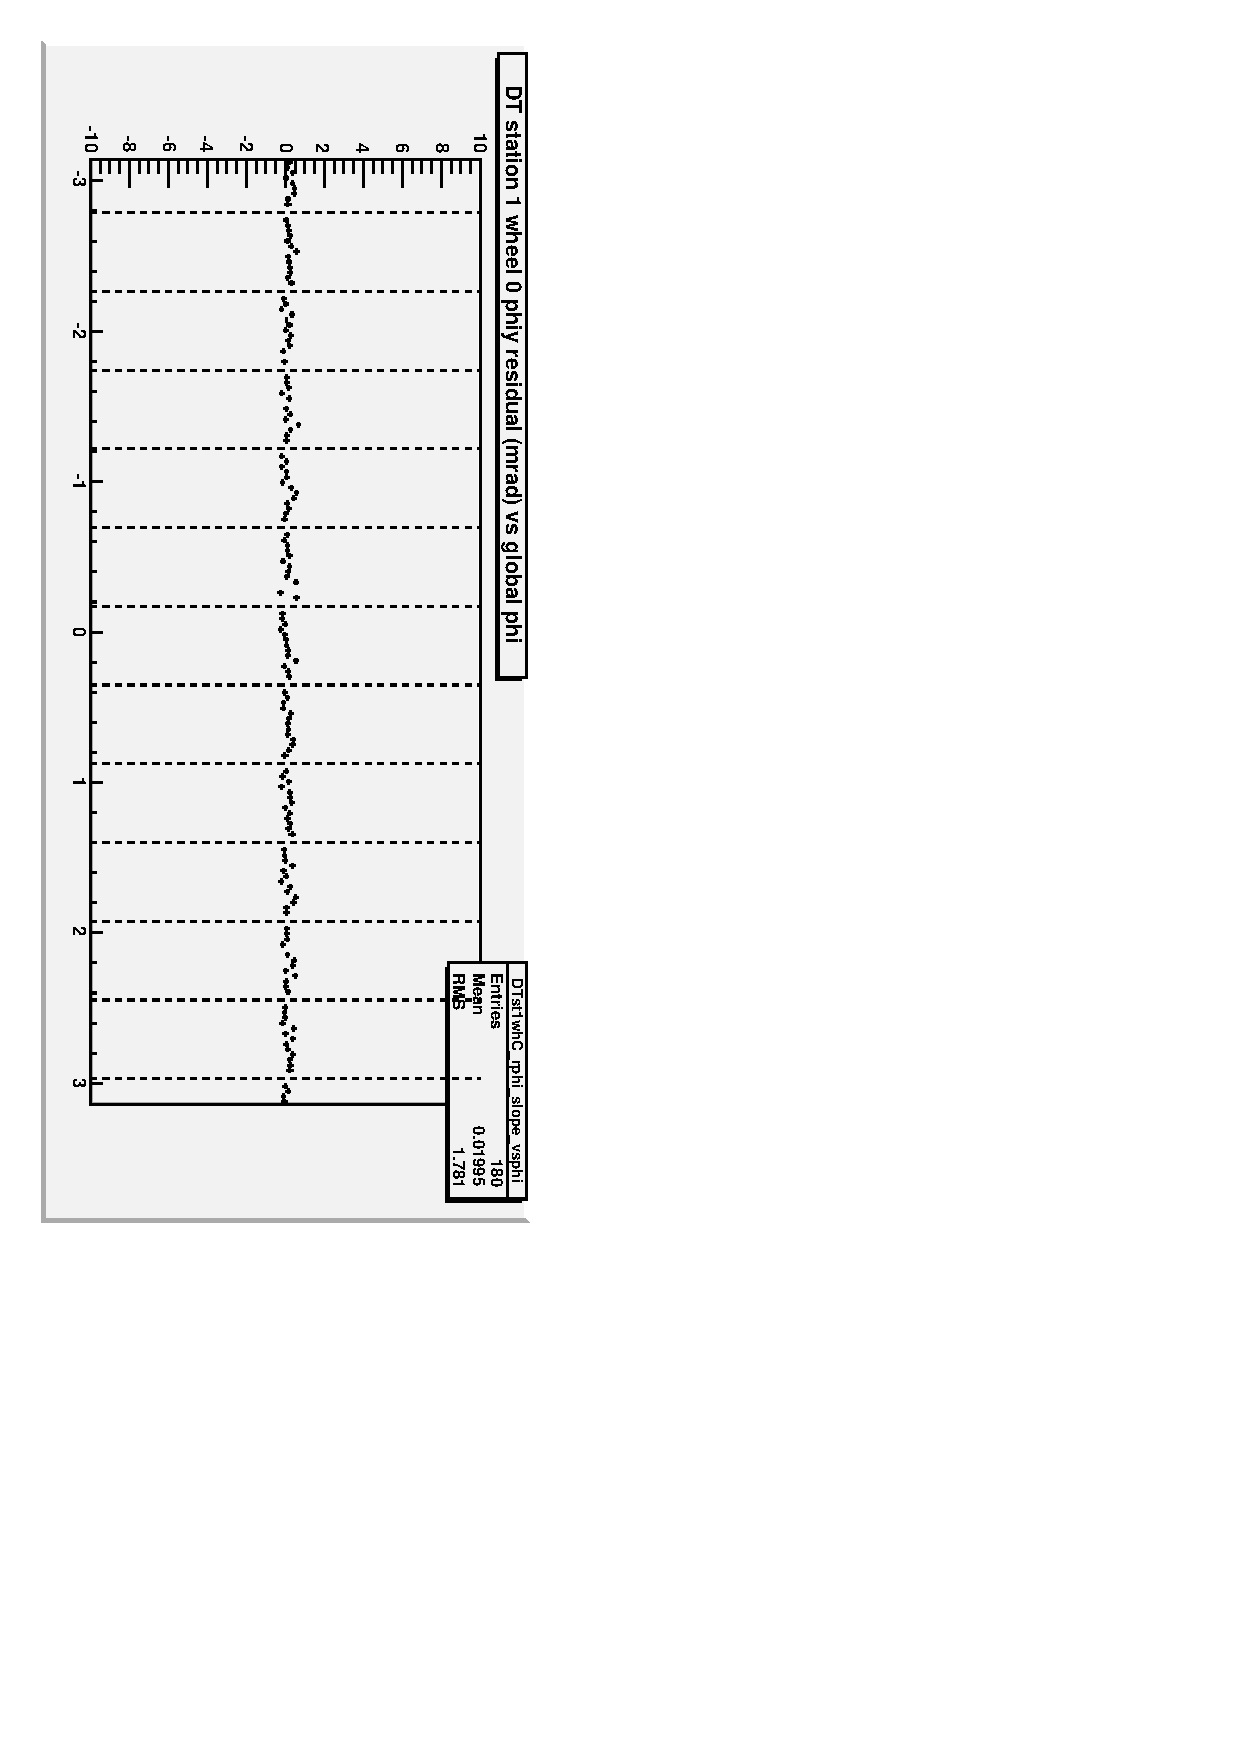
\includegraphics[height=\linewidth, angle=90]{possible_acoplanarity_idealmc.pdf}
\end{frame}

%% \begin{frame}
%% \frametitle{Outline}
%% \begin{itemize}\setlength{\itemsep}{0.75 cm}
%% \item 
%% \end{itemize}
%% %% \hspace{-0.83 cm} \textcolor{darkblue}{\Large Outline2}
%% \end{frame}

%% \section*{First section}
%% \begin{frame}
%% \begin{center}
%% \Huge \textcolor{blue}{First section}
%% \end{center}
%% \end{frame}

\begin{frame}
\frametitle{Conclusions}

\begin{itemize}
\item Most important addition to alignment procedure: $\phi_y$ angles
\item Other improvements:
\begin{itemize}
\item combined fits to manage correlations among parameters \\ (I looked at all of them: none of them ``went wild'')
\item CSCs can, in principle, be aligned, which is an important step toward using this algorithm with standAloneMuons
\item (this is the 3\_1\_X MuonAlignmentAlgorithms update)
\end{itemize}
\item Zoomed in on the surprising feature: $\phi_y$ measurements are not constant across the chamber face
\begin{itemize}
\item it's real, and likely related to the outstanding ``sawtooth'' problem
\item short-term: algorithm aligns the central $\phi_y \to 0$, while we (with DT-DPG) see if this helps to solve the sawtooth problem
\end{itemize}
\end{itemize}

\label{numpages}
\end{frame}

\end{document}
